%
%Academic CV LaTeX Template
% Author: Dubasi Pavan Kumar
% LinkedIn: https://www.linkedin.com/in/im-pavankumar/
% License: MIT
%
% For errors, suggestions, or improvements, please contact:
% Email: pavankumard.pg19.ma@nitp.ac.in
%



\documentclass[a4paper,11pt]{article}

% Package imports
\usepackage{latexsym}
\usepackage{xcolor}
\usepackage{float}
\usepackage{ragged2e}
\usepackage[empty]{fullpage}
\usepackage{wrapfig}
\usepackage{lipsum}
\usepackage{tabularx}
\usepackage{titlesec}
\usepackage{geometry}
\usepackage{marvosym}
\usepackage{verbatim}
\usepackage{enumitem}
\usepackage{fancyhdr}
\usepackage{multicol}
\usepackage{graphicx}
\usepackage{cfr-lm}
\usepackage[T1]{fontenc}
\usepackage{fontawesome5}
\usepackage{gensymb}%for the degree symbol

% Color definitions
\definecolor{darkblue}{RGB}{0,0,139}

% Page layout
\setlength{\multicolsep}{0pt} 
\pagestyle{fancy}
\fancyhf{} % clear all header and footer fields
\fancyfoot{}
\renewcommand{\headrulewidth}{0pt}
\renewcommand{\footrulewidth}{0pt}
\geometry{left=1.4cm, top=0.8cm, right=1.2cm, bottom=1cm}
\setlength{\footskip}{5pt} % Addressing fancyhdr warning

% Hyperlink setup (moved after fancyhdr to address warning)
\usepackage[hidelinks]{hyperref}
\hypersetup{
    colorlinks=true,
    linkcolor=darkblue,
    filecolor=darkblue,
    urlcolor=darkblue,
}

% Custom box settings
\usepackage[most]{tcolorbox}
\tcbset{
    frame code={},
    center title,
    left=0pt,
    right=0pt,
    top=0pt,
    bottom=0pt,
    colback=gray!20,
    colframe=white,
    width=\dimexpr\textwidth\relax,
    enlarge left by=-2mm,
    boxsep=4pt,
    arc=0pt,outer arc=0pt,
}

% URL style
\urlstyle{same}

% Text alignment
\raggedright
\setlength{\tabcolsep}{0in}

% Section formatting
\titleformat{\section}{
  \vspace{-4pt}\scshape\raggedright\large
}{}{0em}{}[\color{black}\titlerule \vspace{-7pt}]

% Custom commands
\newcommand{\resumeItem}[2]{
  \item{
    \textbf{#1}{\hspace{0.5mm}#2 \vspace{-0.5mm}}
  }
}

\newcommand{\resumePOR}[3]{
\vspace{0.5mm}\item
    \begin{tabular*}{0.97\textwidth}[t]{l@{\extracolsep{\fill}}r}
        \textbf{#1}\hspace{0.3mm}#2 & \textit{\small{#3}} 
    \end{tabular*}
    \vspace{-2mm}
}

\newcommand{\resumeSubheading}[4]{
\vspace{0.5mm}\item
    \begin{tabular*}{0.98\textwidth}[t]{l@{\extracolsep{\fill}}r}
        \textbf{#1} & \textit{\footnotesize{#4}} \\
        \textit{\footnotesize{#3}} &  \footnotesize{#2}\\
    \end{tabular*}
    \vspace{-2.4mm}
}

\newcommand{\resumeProject}[4]{
\vspace{0.5mm}\item
    \begin{tabular*}{0.98\textwidth}[t]{l@{\extracolsep{\fill}}r}
        \textbf{#1} & \textit{\footnotesize{#3}} \\
        \footnotesize{\textit{#2}} & \footnotesize{#4}
    \end{tabular*}
    \vspace{-2.4mm}
}

\newcommand{\resumeSubItem}[2]{\resumeItem{#1}{#2}\vspace{-4pt}}

\renewcommand{\labelitemi}{$\vcenter{\hbox{\tiny$\bullet$}}$}
\renewcommand{\labelitemii}{$\vcenter{\hbox{\tiny$\circ$}}$}

\newcommand{\resumeSubHeadingListStart}{\begin{itemize}[leftmargin=*,labelsep=1mm]}
\newcommand{\resumeHeadingSkillStart}{\begin{itemize}[leftmargin=*,itemsep=1.7mm, rightmargin=2ex]}
\newcommand{\resumeItemListStart}{\begin{itemize}[leftmargin=*,labelsep=1mm,itemsep=0.5mm]}

\newcommand{\resumeSubHeadingListEnd}{\end{itemize}\vspace{2mm}}
\newcommand{\resumeHeadingSkillEnd}{\end{itemize}\vspace{-2mm}}
\newcommand{\resumeItemListEnd}{\end{itemize}\vspace{-2mm}}
\newcommand{\cvsection}[1]{%
\vspace{2mm}
\begin{tcolorbox}
    \textbf{\large #1}
\end{tcolorbox}
    \vspace{-4mm}
}

\newcolumntype{L}{>{\raggedright\arraybackslash}X}%
\newcolumntype{R}{>{\raggedleft\arraybackslash}X}%
\newcolumntype{C}{>{\centering\arraybackslash}X}%

% Commands for icon sizing and positioning
\newcommand{\socialicon}[1]{\raisebox{-0.05em}{\resizebox{!}{1em}{#1}}}
\newcommand{\ieeeicon}[1]{\raisebox{-0.3em}{\resizebox{!}{1.3em}{#1}}}

% Font options
\newcommand{\headerfonti}{\fontfamily{phv}\selectfont} % Helvetica-like (similar to Arial/Calibri)
\newcommand{\headerfontii}{\fontfamily{ptm}\selectfont} % Times-like (similar to Times New Roman)
\newcommand{\headerfontiii}{\fontfamily{ppl}\selectfont} % Palatino (elegant serif)
\newcommand{\headerfontiv}{\fontfamily{pbk}\selectfont} % Bookman (readable serif)
\newcommand{\headerfontv}{\fontfamily{pag}\selectfont} % Avant Garde-like (similar to Trebuchet MS)
\newcommand{\headerfontvi}{\fontfamily{cmss}\selectfont} % Computer Modern Sans Serif
\newcommand{\headerfontvii}{\fontfamily{qhv}\selectfont} % Quasi-Helvetica (another Arial/Calibri alternative)
\newcommand{\headerfontviii}{\fontfamily{qpl}\selectfont} % Quasi-Palatino (another elegant serif option)
\newcommand{\headerfontix}{\fontfamily{qtm}\selectfont} % Quasi-Times (another Times New Roman alternative)
\newcommand{\headerfontx}{\fontfamily{bch}\selectfont} % Charter (clean serif font)

\begin{document}
\headerfontiii

% Header
\begin{center}
    {\Huge\textbf{Mitchell Tillman, PhD}}
\end{center}
\vspace{-6mm}

\begin{center}
    \small{
    +1-847-687-3787 | \href{mailto:mtillman14@gmail.com}{mtillman14@gmail.com}
    % \href{https://www.mathworks.com/matlabcentral/profile/authors/16297861}{MATLAB File Exchange}
    }
\end{center}
\vspace{-6mm}

\begin{center}
    \small{
    \socialicon{\faLinkedin} \href{https://www.linkedin.com/in/mitchelltillman/}{mitchelltillman} | 
    \socialicon{\faGithub} \href{https://github.com/mtillman14}{mtillman14} | 
    \ieeeicon{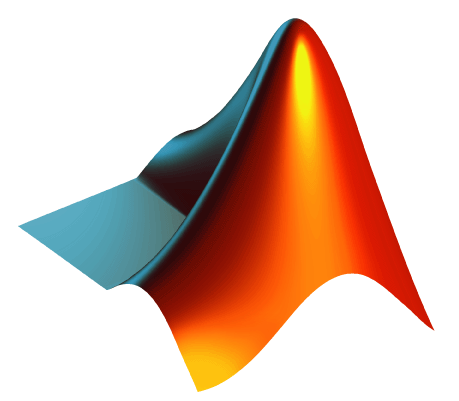
\includegraphics[height=1.3em]{matlab_icon.png}} \href{https://www.mathworks.com/matlabcentral/profile/authors/16297861}{Mitchell Tillman} |
    \socialicon{\faTwitter} \href{https://x.com/tillmn8r}{tillmn8r}
    }
\end{center}
\vspace{-6mm}
\begin{center}
    \small{Gurnee, IL USA 60031}
\end{center}

\vspace{-4mm}

\section{\textbf{Objective}}
\vspace{1mm}
% \small{
Ph.D. seeking a data science position to leverage my academic research experience deriving actionable insights from complex datasets. I am passionate about developing tools to facilitate new discoveries in biomedical data.
}
% \small{
Seeking a sports biomechanist position, leveraging my expertise in analyzing human movement. Aiming to contribute to innovative projects at the intersection of biomechanics, motor control, and data science with the goal of improving movement performance. I am passionate about developing tools to facilitate new discoveries in biomechanical data, and I'm looking to grow my analytical skills and translate them to player development.
}
% \small{
Seeking a challenging position in biomechanics to leverage my expertise in analyzing human movement. Aiming to contribute to innovative projects at the intersection of biomechanics, motor control, data science, and practical problem-solving with the goal of improving movement performance. I am passionate about developing tools to facilitate new discoveries in biomechanical data, and I'm looking to learn more about data science practices in a production setting.
}
% \small{
Ph.D. in biomedical engineering seeking a challenging post-doctoral research position. Aiming to contribute to innovative projects at the intersection of biomechanics, motor control, data science, and practical problem-solving with the goal of improving movement rehabilitation and performance. I am also passionate about developing tools to facilitate new discoveries in biomechanical data.
}
\small{
Ph.D. in biomedical engineering seeking a challenging and rewarding role as a biomechanist. My Ph.D. focused on the whole-body biomechanics of gait, and I aim to leverage that training to improve patients' quality of life. I am also passionate about developing tools to facilitate new discoveries in biomechanical data.
}
% \small{
Ph.D. in Biomedical Engineering with extensive experience in data analysis and statistical modeling seeking to join Abbott as a Staff Data Scientist. Aiming to leverage expertise in Python, R, and data analysis to contribute to the optimization of medical devices in diabetes care.
}
\vspace{-2mm}



% \section{\textbf{Experience}}
% \vspace{-0.4mm}
%   \resumeSubHeadingListStart
%   \resumeSubheading
%       {{Company A [\href{https://www.companya.com}{\faIcon{globe}}]}}{City, Country}
%       {Job Title A}{Month Year - Month Year}
%       \resumeItemListStart
%         \item Developed [specific achievement] achieving [specific metric] in [specific area]
%         \item Implemented [technology/method], enhancing [specific aspect] by [specific percentage]
%         \item Conducted analysis on [specific data], identifying [key findings]
%         \item Presented findings at [specific event], receiving [specific recognition]
%       \resumeItemListEnd 
%   \resumeSubheading
%     {Company B [\href{https://www.companyb.com}{\faIcon{globe}}]}{Remote}
%     {Job Title B}{Month Year - Month Year}
%     \resumeItemListStart
%       \item Engineered a [specific system/model], improving [specific metric] by [percentage]
%       \item Developed [specific tool/method], increasing [specific aspect] by [percentage]
%       \item Implemented [specific system], reducing [specific metric] by [percentage]
%       \item Conducted [specific test/analysis] to validate [specific aspect]
%     \resumeItemListEnd
%   \resumeSubHeadingListEnd
% \vspace{-6mm}

\section{\textbf{Education}}
\vspace{-0.4mm}
\resumeSubHeadingListStart

\resumeSubheading
{Stevens Institute of Technology}{Hoboken, NJ USA}
{\parbox[t]{0.7\linewidth}{Ph.D. Mechanics of Whole-Body Balance and Momentum Control During \newline Straight-Line Gait and 90\degree~Turns}}{Oct 2024}
\resumeItemListStart
\item GPA: 4.00/4.00
\resumeItemListEnd

\resumeSubheading
{Purdue University}{West Lafayette, IN USA}
{\parbox[t]{0.8\linewidth}{M.S. Effects of Past and Future Motor Events on Present Motor Stability, \newline and Relationships with Motor and Cognitive Flexibility}}{May 2019}
\resumeItemListStart
\item GPA: 3.59/4.00
\resumeItemListEnd

\resumeSubheading
{Purdue University}{West Lafayette, IN USA}
{B.S. Movement \& Sports Sciences}{May 2018}
\resumeItemListStart
\item GPA: 3.12/4.00
\resumeItemListEnd

\resumeSubHeadingListEnd
\vspace{-6mm}

\section{\textbf{Projects}}
\vspace{-0.4mm}
\resumeSubHeadingListStart

\resumeProject
  {Research OS: A tool for shareable data analysis (in development)}
  {Tools: Python, SQLite}
  {Sep 2021 - Present}
  {{}\href{https://github.com/ResearchOS/ResearchOS}{\textcolor{darkblue}{\faGithub}}}
\resumeItemListStart
  \item pip install-able Python packages by default means that every data analysis is easily publicly shareable
  \item Workflow orchestration, data pipeline management, and many other tools to facilitate interacting with and learning from data
  \item I have been developing the concept for years, gaining experience with MATLAB GUI, Python, SQLite, and config files (JSON, TOML) through multiple implementations
  \item Current and likely final implementation is CLI-based Python scripts with TOML configuration files
  \item Experience publishing the package to test PyPi
\resumeItemListEnd

\resumeProject
  {Development of real-time auditory biofeedback to assist balance}
  {Tools: MATLAB, Optitrack motion capture, MaxMSP, Open Sound Control networking protocol}
  {2019 - 2022}
  {}
  % {{}\href{https://github.com/your-username/project-b}{\textcolor{darkblue}{\faGithub}}}
\resumeItemListStart
  \item Developed the first prototype of a system that converts motion capture data to audio in real time ($\sim$20 ms latency)
  \item Tested older adults' understanding and device useability qualitatively with surveys and interviews
  \item Three of five young adults showed improvements in one legged standing balance with vs. without the device 
\resumeItemListEnd

% \resumeProject
%   {Split-belt treadmill symmetry index return to baseline calculations}
%   {Tools: MATLAB}
%   {}
%   {}
%   % {{}\href{https://github.com/your-username/project-b}{\textcolor{darkblue}{\faGithub}}}
% \resumeItemListStart
%   \item I analyzed the "symmetry index" data (measures left and right step length similarity) that Dr. Ray Lin at Seton Hall University collected on older adults walking on a split-belt treadmill
%   \item My responsibilities were to identify the features in the symmetry index timeseries to establish when the left and right belt speeds diverged, and to quantify how many steps it took for the symmetry index to return to plateau
% \resumeItemListEnd

\resumeProject
  {\parbox[t]{0.75\linewidth}{Dissertation Research: Quantifying balance and momentum control during turns while walking in healthy young and older adults}}
  {Tools: MATLAB, Optitrack motion capture}
  {2021 - 2024}
  {}
  % {{}\href{https://github.com/your-username/project-b}{\textcolor{darkblue}{\faGithub}}}
\resumeItemListStart
  \item Collected motion capture and force plate data on over 50 young and older adult participants walking and turning
  \item Developed a MATLAB data analysis pipeline for custom data analyses based on person-specific biomechanical models, including bespoke visualizations and data-driven videos
  \item Designed the data analysis pipeline to scale by minimizing the data in memory, and implemented rule-based data subsetting for improved flexibility of use
  \item Published three first author journal articles, projects which I led from experiment design through data analysis and writing the manuscript
\resumeItemListEnd

\resumeSubHeadingListEnd

\section{\textbf{Selected Publications}}
\vspace{0.2mm}
\small{
\begin{enumerate}[leftmargin=*, labelsep=0.5em, align=left, widest={[\textbf{S.1}]}, itemindent=0em, label={\textbf{[\arabic*]}]}]
\item[\textbf{[1]}] Tillman et al. (2024). \href{https://doi.org/10.1186/s12984-024-01437-3}{\textbf{Healthy older adults generate transverse-plane momenta required for 90 degree turns during the same phases of gait as in straight-line gait}}. \textit{J. of NeuroEng and Rehab}, 21:145, DOI: 10.1186/s12984-024-01437-3

\item[\textbf{[2]}] Tillman et al. (2020). \href{https://dl.acm.org/doi/10.1145/3401956.3404244}{\textbf{Real-Time Optical Motion Capture Balance Sonification System}}. \textit{ACM Int. Conf. Proc. Series}, DOI: 10.1145/3401956.3404244

% \item[\textbf{[2]}] Tillman et al. (2022). \href{https://doi.org/10.1016/j.jbiomech.2022.111206}{\textbf{Frontal plane balance during pre-planned and late-cued 90 degree turns while walking}}. \textit{J Biomechanics}, DOI: 10.1016/j.jbiomech.2022.111206

\item[\textbf{[3]}] Tillman et al. (2018). \href{https://doi.org/10.1007/s00221-018-5333-0}{\textbf{Expectation of movement generates contrasting changes in multifinger synergies in young and older adults}}. \textit{Exp. Brain Research}, DOI: 10.1007/s00221-018-5333-0
\end{enumerate}
}

\section{\textbf{Skills}}
\vspace{-0.4mm}
 \resumeHeadingSkillStart
  \resumeSubItem{Programming Languages (in order of experience):}
    {MATLAB, Python, R, SQL, bash}
  % \resumeSubItem{Web Technologies:}
  %   {Technology 1, Technology 2, Technology 3, Technology 4, Technology 5}
  \resumeSubItem{Database Systems:}
    {SQLite}
%   \resumeSubItem{Data Science \& Machine Learning:}
%     {Tool 1, Tool 2, Tool 3, Tool 4, Tool 5, Tool 6}
% \resumeSubItem{Cloud Technologies:}
%     {Cloud Platform 1, Cloud Platform 2, Cloud Platform 3}
  \resumeSubItem{DevOps \& Version Control:}
    {Git, GitHub}
  % \resumeSubItem{Specialized Area:}
  %   {Biomechanics, Motor control, Motion capture}
  \resumeSubItem{Mathematical \& Statistical Tools:}
    {regression, ANOVA, k-means cluster analysis, linear mixed models}
  \resumeSubItem{Other Tools \& Technologies:}
    {DeepLabCut (markerless motion capture), DeepLabCut Live, MaxMSP}
  \resumeSubItem{Research Skills:}{Experiment Design, Data Collection, Data Analysis, Pipeline Development, Biomechanics}
 \resumeHeadingSkillEnd

\section{\textbf{Honors and Awards}}
\vspace{-0.4mm}
\resumeSubHeadingListStart

\resumeProject
  {Doctoral Excellence Fellowship}
  {Stevens Institute of Technology}
  {May 2023}
  {}
\resumeItemListStart
  \item Full tuition and stipend awarded for one academic year based on excellence in activities through the Ph.D. program
\resumeItemListEnd

% \resumeProject
%   {Robert Crooks Stanley Fellowship}
%   {Robert Crooks Stanley Graduate Fellowship Committee}
%   {Aug 2022}
%   {{}\href{https://www.stevens.edu/academics/graduate-study/graduate-funding/assistantships-and-fellowships\#scholarships-fellowships}{\textcolor{darkblue}{\faIcon{globe}}}}
% \resumeItemListStart
%   \item Awarded to researchers exhibiting the qualities of industrialism upheld by the committee
%   % \item Impact or recognition associated with the award
% \resumeItemListEnd

\resumeProject
  {Outstanding Masters Student in the College of Health and Human Sciences}
  {Purdue University}
  {May 2019}
  {}
\resumeItemListStart
  \item \$500 awarded for outstanding achievements in original research 
  % \item Skills or abilities demonstrated through this achievement
\resumeItemListEnd

\resumeSubHeadingListEnd

\vspace{-6mm}
\section{\textbf{Leadership Experience}}
\vspace{-0.4mm}
\resumeSubHeadingListStart
\resumeProject
  {Project Team Lead}
  {NJ Governor's STEM Scholars}
  {Sep 2021 - May 2022}
  {{}\href{https://www.govstemscholars.com/scholars}{\textcolor{darkblue}{\faIcon{globe}}}}
\resumeItemListStart
  \item Led a team of 10 high school students in designing, implementing, and testing a real-time auditory biofeedback system to improve balance using open source software 
  \item Received mentorship from Dr. Gary Kane, a core developer of DeepLabCut Live, to implement the auditory biofeedback system
  % \item Evaluated the efficacy of the auditory biofeedback system by collecting and analyzing data of 10 participants' balance while standing still with and without auditory biofeedback.
\resumeItemListEnd

\resumeProject
  {Secretary, Graduate Biomedical Engineering Society}
  {Stevens Institute of Technology}
  {Aug 2021 - Aug 2022}
  {{}\href{https://ducklink.stevens.edu/gbmes/home/}{\textcolor{darkblue}{\faIcon{globe}}}}
\resumeItemListStart
  \item Instituted biweekly graduate student-led department seminars that are still ongoing
  \item Hosted career development events for the BME department, including negotiating funding from the school for the even to secure food and external speakers.
\resumeItemListEnd

\resumeSubHeadingListEnd

\vspace{-6mm}

\section{\textbf{Volunteer Experience}}
\vspace{-0.4mm}
\resumeSubHeadingListStart
\resumeProject
  {Student Committee Member}
  {American Society of Biomechanics (ASB)}
  {2022 - 2024}
  {{}\href{https://asbweb.org}{\textcolor{darkblue}{\faIcon{globe}}}}
\resumeItemListStart
  \item Helped plan the student-oriented sessions at the international ASB conference, such as roundtable discussions, student meetups, etc.
  \item Secured \$5,000 sponsorship from Optitrack for two consecutive years for student night out at the conference.
\resumeItemListEnd

\resumeProject
  {National Biomechanics Day}
  {The Biomechanics Initiative at Stevens Institute of Technology}
  {2020 - 2023}
  {{}[\href{https://thebiomechanicsinitiative.org}{\textcolor{darkblue}{\faIcon{globe}}}]}
\resumeItemListStart
  \item Introduced middle school through high school aged children to the field of biomechanics through fun interactive activities such as dancing with EMG sensors to visualize muscle activity, etc.
\resumeItemListEnd

\resumeSubHeadingListEnd
\vspace{-6mm}

\section{\textbf{Professional Memberships}}
\vspace{-0.4mm}
\resumeSubHeadingListStart
\resumePOR{American Society of Biomechanics}
    {}
    {2017 - Present}
\resumePOR{International Society of Posture \& Gait Research}
    {}
    {2023-2024}
\resumePOR{Graduate Biomedical Engineering Society}
    {}
    {2021-2022}
\resumePOR{Society for Neuroscience}
    {}
    {2019, 2023}

\resumeSubHeadingListEnd
\vspace{-6mm}

% \section{\textbf{Certifications}}
% \vspace{-0.2mm}
% \resumeSubHeadingListStart
% \resumePOR{}{\href{https://certification-link-a.com}{
% \textbf{Certification A}
% }}{Month Year}
% \resumePOR{}{
% \textbf{Certifying Body:} {{\href{https://certification-link-b.com}{Certification B}}}}{Month Year}
% \resumePOR{}{
% \textbf{Certifying Body:} {{\href{https://certification-link-c.com}{Certification C}}}}{Month Year}
% \resumePOR{}{\href{https://certification-link-d.com}{
% \textbf{Certification D}
% }}{Month Year}

% \resumeSubHeadingListEnd
% \vspace{-6mm}

% \section{\textbf{Additional Information}}
% \vspace{-0.4mm}
% \small{
% \textbf{Languages:} English (Native), Spanish (Fluent)

% \textbf{Interests:} Open source software, data analysis tools, martial arts
% }
% \vspace{-4mm}


% \section{\textbf{References}}
% \vspace{-0.2mm}
% \small{
% \begin{enumerate}[leftmargin=*,labelsep=2mm]
% \item \textbf{Dr. Antonia Zaferiou}\\
%    Assistant Professor, Biomedical Engineering\\
%    Stevens Institute of Technology\\
%    Email: antonia.zaferiou@stevens.edu\\
%    Phone: +1-201-216-3662\\
%    \textit{Relationship: Ph.D. Supervisor}

% \item \textbf{Dr. Satyajit Ambike}\\
%    Associate Professor, Health \& Kinesiology\\
%    Purdue University\\
%    Email: sambike@purdue.edu\\
%    Phone: +1-614-209-8407\\
%    \textit{Relationship: M.S. Supervisor}

% \item \textbf{Dr. Sean Sanford}\\
%    Senior Test Engineer\\
%    Medtronic\\
%    Email: sean.sanford2@medtronic.com\\
%    Phone: +1-480-824-8167\\
%    \textit{Relationship: Former Colleague}
% \end{enumerate}
% }

\section{\textbf{References}}
\vspace{-0.2mm}
\small{
\begin{multicols}{2}
\raggedcolumns
\textbf{Dr. Antonia Zaferiou}\\
Assistant Professor, Biomedical Engineering\\
Stevens Institute of Technology\\
Email: antonia.zaferiou@stevens.edu\\
Phone: +1-201-216-3662\\
\textit{Relationship: Ph.D. Supervisor}

\vspace{5mm}

\textbf{Dr. Satyajit Ambike}\\
Associate Professor, Health \& Kinesiology\\
Purdue University\\
Email: sambike@purdue.edu\\
Phone: +1-614-209-8407\\
\textit{Relationship: M.S. Supervisor}

\columnbreak

\vspace{5mm}

\textbf{Dr. Sean Sanford}\\
Senior Test Engineer\\
Medtronic\\
Email: sean.sanford2@medtronic.com\\
Phone: +1-480-824-8167\\
\textit{Relationship: Former Colleague}

\vspace{5mm}

\textbf{Nathaniel Bechhofer}\\
CEO\\
FormToFile\\
Email: nathanielbechhofer@trovbase.com\\
Phone: +1-845-570-1518\\
\textit{Relationship: Mentor and Industry Collaborator}
\end{multicols}
}

\end{document}